% This is "sig-alternate.tex" V1.9 April 2009
% This file should be compiled with V2.4 of "sig-alternate.cls" April 2009
%
% This example file demonstrates the use of the 'sig-alternate.cls'
% V2.4 LaTeX2e document class file. It is for those submitting
% articles to ACM Conference Proceedings WHO DO NOT WISH TO
% STRICTLY ADHERE TO THE SIGS (PUBS-BOARD-ENDORSED) STYLE.
% The 'sig-alternate.cls' file will produce a similar-looking,
% albeit, 'tighter' paper resulting in, invariably, fewer pages.
%
% ----------------------------------------------------------------------------------------------------------------
% This .tex file (and associated .cls V2.4) produces:
%       1) The Permission Statement
%       2) The Conference (location) Info information
%       3) The Copyright Line with ACM data
%       4) NO page numbers
%
% as against the acm_proc_article-sp.cls file which
% DOES NOT produce 1) thru' 3) above.
%
% Using 'sig-alternate.cls' you have control, however, from within
% the source .tex file, over both the CopyrightYear
% (defaulted to 200X) and the ACM Copyright Data
% (defaulted to X-XXXXX-XX-X/XX/XX).
% e.g.
% \CopyrightYear{2007} will cause 2007 to appear in the copyright line.
% \crdata{0-12345-67-8/90/12} will cause 0-12345-67-8/90/12 to appear in the copyright line.
%
% ---------------------------------------------------------------------------------------------------------------
% This .tex source is an example which *does* use
% the .bib file (from which the .bbl file % is produced).
% REMEMBER HOWEVER: After having produced the .bbl file,
% and prior to final submission, you *NEED* to 'insert'
% your .bbl file into your source .tex file so as to provide
% ONE 'self-contained' source file.
%
% ================= IF YOU HAVE QUESTIONS =======================
% Questions regarding the SIGS styles, SIGS policies and
% procedures, Conferences etc. should be sent to
% Adrienne Griscti (griscti@acm.org)
%
% Technical questions _only_ to
% Gerald Murray (murray@hq.acm.org)
% ===============================================================
%
% For tracking purposes - this is V1.9 - April 2009

\documentclass{sig-alternate}
  \pdfpagewidth=8.5truein
  \pdfpageheight=11truein

\begin{document}
%
% --- Author Metadata here ---
\conferenceinfo{Data Mining Course}{June, 2015, Shanghai, China.}
\CopyrightYear{2015} % Allows default copyright year (2002) to be over-ridden - IF NEED BE.
\crdata{}  % Allows default copyright data (X-XXXXX-XX-X/XX/XX) to be over-ridden.
% --- End of Author Metadata ---

\title{Predicting PM2.5 Value in Future}
%
% You need the command \numberofauthors to handle the 'placement
% and alignment' of the authors beneath the title.
%
% For aesthetic reasons, we recommend 'three authors at a time'
% i.e. three 'name/affiliation blocks' be placed beneath the title.
%
% NOTE: You are NOT restricted in how many 'rows' of
% "name/affiliations" may appear. We just ask that you restrict
% the number of 'columns' to three.
%
% Because of the available 'opening page real-estate'
% we ask you to refrain from putting more than six authors
% (two rows with three columns) beneath the article title.
% More than six makes the first-page appear very cluttered indeed.
%
% Use the \alignauthor commands to handle the names
% and affiliations for an 'aesthetic maximum' of six authors.
% Add names, affiliations, addresses for
% the seventh etc. author(s) as the argument for the
% \additionalauthors command.
% These 'additional authors' will be output/set for you
% without further effort on your part as the last section in
% the body of your article BEFORE References or any Appendices.

\numberofauthors{1} %  in this sample file, there are a *total*
% of EIGHT authors. SIX appear on the 'first-page' (for formatting
% reasons) and the remaining two appear in the \additionalauthors section.
%
\author{
% You can go ahead and credit any number of authors here,
% e.g. one 'row of three' or two rows (consisting of one row of three
% and a second row of one, two or three).
%
% The command \alignauthor (no curly braces needed) should
% precede each author name, affiliation/snail-mail address and
% e-mail address. Additionally, tag each line of
% affiliation/address with \affaddr, and tag the
% e-mail address with \email.
%
% 1st. author
\alignauthor Zhaowei Tan\titlenote{This author is the
one who did all the really hard work. All the codes, methods and approaches are written or designed by the author. I will EXPLICITLY point out when some work mentioned in the paper is not done by this author, for example, an open source program.}\\
       \affaddr{5120309701}\\
       \affaddr{IEEE Honor Class}\\
       \affaddr{Shanghai Jiao Tong University}\\
       \affaddr{Shanghai, China}\\
       \email{tanzw94@gmail.com}
}
% There's nothing stopping you putting the seventh, eighth, etc.
% author on the opening page (as the 'third row') but we ask,
% for aesthetic reasons that you place these 'additional authors'
% in the \additional authors block, viz.

\date{5 July 2015}
% Just remember to make sure that the TOTAL number of authors
% is the number that will appear on the first page PLUS the
% number that will appear in the \additionalauthors section.


\maketitle
\begin{abstract}
PM2.5 is a critical environmental issue being discussed nowadays; when the amount of PM2.5 reaches a certain level, it does harm to both human beings and the whole environment. Therefore, predicting the value of PM2.5 becomes one of the critical problems, for this will allow citizens and the departments concerned to implement corresponding measures ahead of time. In this paper, I use data mining techniques to solve two problems concerning PM2.5. The first is to predict the PM2.5 value of the next time session while the other is to determine the PM2.5 pollution level category of the next day. I mainly use neural network combined with some other models to solve the two problems and the experimental results indicates good performance. Finally, I discuss some possible approaches to refine the process to end this paper.
\end{abstract}



\keywords{Data Mining, Regression, Classification PM2.5, Health and Environment}

\section{Introduction}
\footnote{This project does not ask us to hand in the source code, but I upload most of the source codes in a Github repository . You can find that in https://github.com/ZhaoweiTan/pm.}We are living on an unhealthy Mother Earth. The industrialization and modernization accommodate us with a better life, while failing to provide a healthier environment. The Partical Pollution(PM) is a rising problem which has drawn more and more attention nowadays. Many websites, like Baidu, put real-time PM value in their frontpages. The general public and the government have been aware of this insidious air pollution, trying to find ways to solve this environmental puzzle.

PM, is a mixture of solids and liquid droplets floating in the air\cite{pm}. Some particles are released directly from a specific source, while others form in complicated chemical reactions in the atmosphere. Particles come in a wide range of sizes. Particles less than or equal to 10 micrometers in diameter are so small that they can get into the lungs, potentially causing serious health problems. Ten micrometers is less than the width of a single human hair.

More specifically, this paper focus on fine particles. Fine particles (PM2.5) are 2.5 micrometers in diameter or smaller, and can only be seen with an electron microscope. Fine particles are produced from all types of combustion, including motor vehicles, power plants, residential wood burning, forest fires, agricultural burning, and some industrial processes. PM2.5 will trigger both negative health effects and environmental effects. For example, it will cause irritation of the eyes, building damage, or even heart attacks.

Considering the destructive effect of PM2.5, predicting the value of PM2.5 becomes a meaningful task. If we can use the past historic data to predict the PM2.5 value of the next hour, or even next day, the public and the departments concerned will be more prompt to make some corresponding measures. For example, if I know that tomorrow will be heavy of PM2.5, I might cancel the football match held outdoors.

In this paper, several machine learning methods are deployed to predict the value or level of PM2.5 in future. The dataset we downloaded from FTP is provided by U.S. Department of State\cite{data}. The dataset consists of various PM2.5 data from different cities in China for several years, and more detailed description of data will be presented in Section 3.1.

The paper is organized as follows. I give the sound description of the problem in Section 2. In Section 3, I present some basic processing and analyzing of the original raw data. In Section 4, multiple machine learning methods are proposed to solve the problems using the data we get. All the experimental results are shown in Section 5, after which I elaborate possible future work in Section 6. Finally, I conclude this paper in Section 7.



\section{Problem Description}
I develop two different problems to solve in this paper.
\newtheorem{theorem}{Promblem}
\begin{theorem}
Given historic data $[X,Y]$, in which $X=[x_{1}^{T},x_{2}^{T},...,x_{n}^{T}]^{T}$, and $Y=[y_1, y_2, ..., y_n]$, where $x_i$ is the historic data series corresponds to the observed data $y_i$. Our goal is to us predict the number $y_t$ when we have observed $x_t$. Therefore, this is a regression problem.
\end{theorem}

Next, I consider a more practical problem. Considering the scenario that you want to plan for tomorrow, the PM level of that day should be taken into account, just like the traditional information like temperature or raining or not. So the next problem is to predict to which level will the next day's average PM2.5 be. The categories here is set according to Air Quality Guide.\cite{level} There are seven categories, Good, Moderate, Unhealthy for Sensitive Groups, Unhealthy, Very Unhealthy, Hazardous and Beyond Index, I use $1$ to $7$ to represent them respectively.

\newtheorem{theorem1}{Promblem}
\begin{theorem}
Given historic data $[X,Y]$, in which $X=[x_{1}^{T},x_{2}^{T},...,x_{n}^{T}]^{T}$, and $Y=[y_1, y_2, ..., y_n]$, where $x_i$ is the historic data series corresponds to the average daily PM2.5 pollution category $y_i \in \{1, 2, 3, 4, 5, 6, 7\}$. Our goal is to us predict the average daily PM2.5 level category $y_t$ when we have observed $x_t$. Therefore, this is a multi-classification problem.
\end{theorem}

After this, I found that the training data is so insufficient so that I modify that a little bit, changing 7 categories into 3, that is, healthy(0-50), moderate(51-100) and unhealthy(>100), respectively. In other words, $y_i \in \{1, 2, 3\}$




\section{Data Analysis and Processing}
After I have defined the scope of this paper and the specific problem description, it is high time that I introduced the dataset and the ways to handle the data. This may highlight the property of the information we get and provide a insight of the approaches we implement to achieve the goal and solve the problems.

\subsection{Data Description}
The dataset we get is provided by U.S. Department of State\cite{data}. In the dataset, we have the PM2.5 data in Beijing, from 2008 to 2014, Chengdu, from 2012 to 2014, Guangzhou, from 2011 to 2014, Shanghai, from 2011 to 2014 and Shenyang, from 2013 to 2014. In each csv sheet, there contains the time of each record and corresponding PM value of that time. Since the Beijing has the most PM2.5 data records, I mostly train the model using Beijing data.

Unfortunately, some data are missing due to several reasons. That makes the time series uncomplete and triggers several difficulties to generate training set, which will be elaborated in Section 3.2. I wrote a simple Python program to get the statistics of all the data.

A brief summary of the data can be found in the Table 1.

\begin{table}[ht]
\centering
\caption{Data Description}
\begin{tabular}{|c|c|c|c|c|}  \hline
City&Year&Missing&All&Missing \\
&&Records&Records&Rate\\ \hline
Beijing&2008&266&5087&5.2\% \\ \hline
Beijing&2009&1981&8760&22.6\% \\ \hline
Beijing&2010&669&8760&7.6\% \\ \hline
Beijing&2011&727&8760&8.3\% \\ \hline
Beijing&2012&489&8784&5.6\% \\ \hline
Beijing&2013&82&8760&9.4\% \\ \hline
Beijing&2014&99&8760&11.3\% \\ \hline \hline
Chengdu&2012&4372&8784&49.8\% \\ \hline
Chengdu&2013&1393&8760&15.9\% \\ \hline
Chengdu&2014&285&8760&3.3\% \\ \hline \hline
Guangzhou&2011&7863&8760&89.8\% \\ \hline
Guangzhou&2012&2249&8784&25.6\% \\ \hline
Guangzhou&2013&384&8760&4.4\% \\ \hline
Guangzhou&2014&669&8760&7.6\% \\ \hline \hline
Shanghai&2011&8683&8760&99.1\% \\ \hline
Shanghai&2012&283&8784&3.2\% \\ \hline
Shanghai&2013&184&8760&2.1\% \\ \hline
Shanghai&2014&136&8760&1.6\% \\ \hline \hline
Shenyang&2013&3374&8760&38.5\% \\ \hline
Shenyang&2014&357&8760&4.1\% \\ \hline \hline
\end{tabular}
\end{table}

\subsection{Training Data Acquisition}
Now that we have the raw data, I shall convert that into the format which can be recognized by MATLAB. I wrote a Python script to do the transformation.

Recall that in the last section, I illustrated that much raw data is missing in the original csv. So in Python script I carefully select the recordings that are available for training, which means I choose the records that has a complete prior PM data, instead of some missing ones.

Considering that every city has a disparate environment and thus the model should be trained within different cities, I henceforth only choose data from Beijing to do this Beijing. Without the lost of generality, the same approaches can be used in other cities, as long as I have sufficient data from that city.

For problem 1, I make an assumption that the PM level will only be related to recent historic data; the data that is far earlier than the predicted time will have little or nothing to do with that time's value. I collect all the records that their past 24-hour data are complete, and have a total of 47407 records altogether in Beijing. I separate them to be my training, cross validation and testing data. Basically, here I harness the AR model, where the dimension of AR model is set to be 24, to train the data and predict the PM value.

 Alternatively, I select another set of features to do the experiment. Instead of only choosing the past hours' data only, I add the same hour's data in the past days into feature space, taking the fact that PM value is probably related to the time in a day into account. So the total dimension is two more than the first one, namely 26.

For problem 2, I calculate the daily average PM2.5 value in Beijing and collect all the records that their past 3-day data are complete. Finally I have a total of 1505 records of data. I separate them to be my training, cross validation and testing data as well .






\section{Learning Approaches}
Two problems are regression problem and classification problems, respectively. So different methods are employed to solve the problems.

Here are several models that I can train to solve the two problems:


For Problem 1:
\begin{itemize}
	\item Linear Regression
    \item Polynomial Regression
	\item Neural Network
    \item ...
\end{itemize}

For Problem 2:
\begin{itemize}
	\item Logistic Regression
    \item Neural Network
    \item Linear Regression
    \item Gaussian Mixture Model
    \item ...
\end{itemize}

We are quite familiar with these methods, so I do not bother introducing these approaches from scratch. Considering the time and my poor laptop configuration, I tried some of these methods, and then show the corresponding result in the next section.




\section{Experimental Results}
My data processing tasks are finished on a 4G memory MacOS X computer. These tasks utilize Python 2.7 scripts. My machine learning problems are solved using a 4G memory Window 7. The version of MATLAB is MATLAB 2013b.

\subsection{Results for Problem 1}
As stated before, due to the constraints of time and other resources, I perform one method to solve the Problem 1, that is the Neural Network, because Neural Network fits the data in a polynomial and thus a better way. Also, the neural network will not take much time for the amount of data is not that much. Thanks to the friendly MATLAB machine learning toolkits\cite{nn}, I avoid writing bunch of codes and debugging for a long time. I set 70\% as the training set, 15\% as the cross validation set, and the rest 15\% as the testing set. The neurons in the hidden layer is set to be 50.

For the model, as was stated in 3.2, I use two sets of features. Their performances are presented in the Figure 1 and Figure 2.

\begin{figure}[ht]
\centering
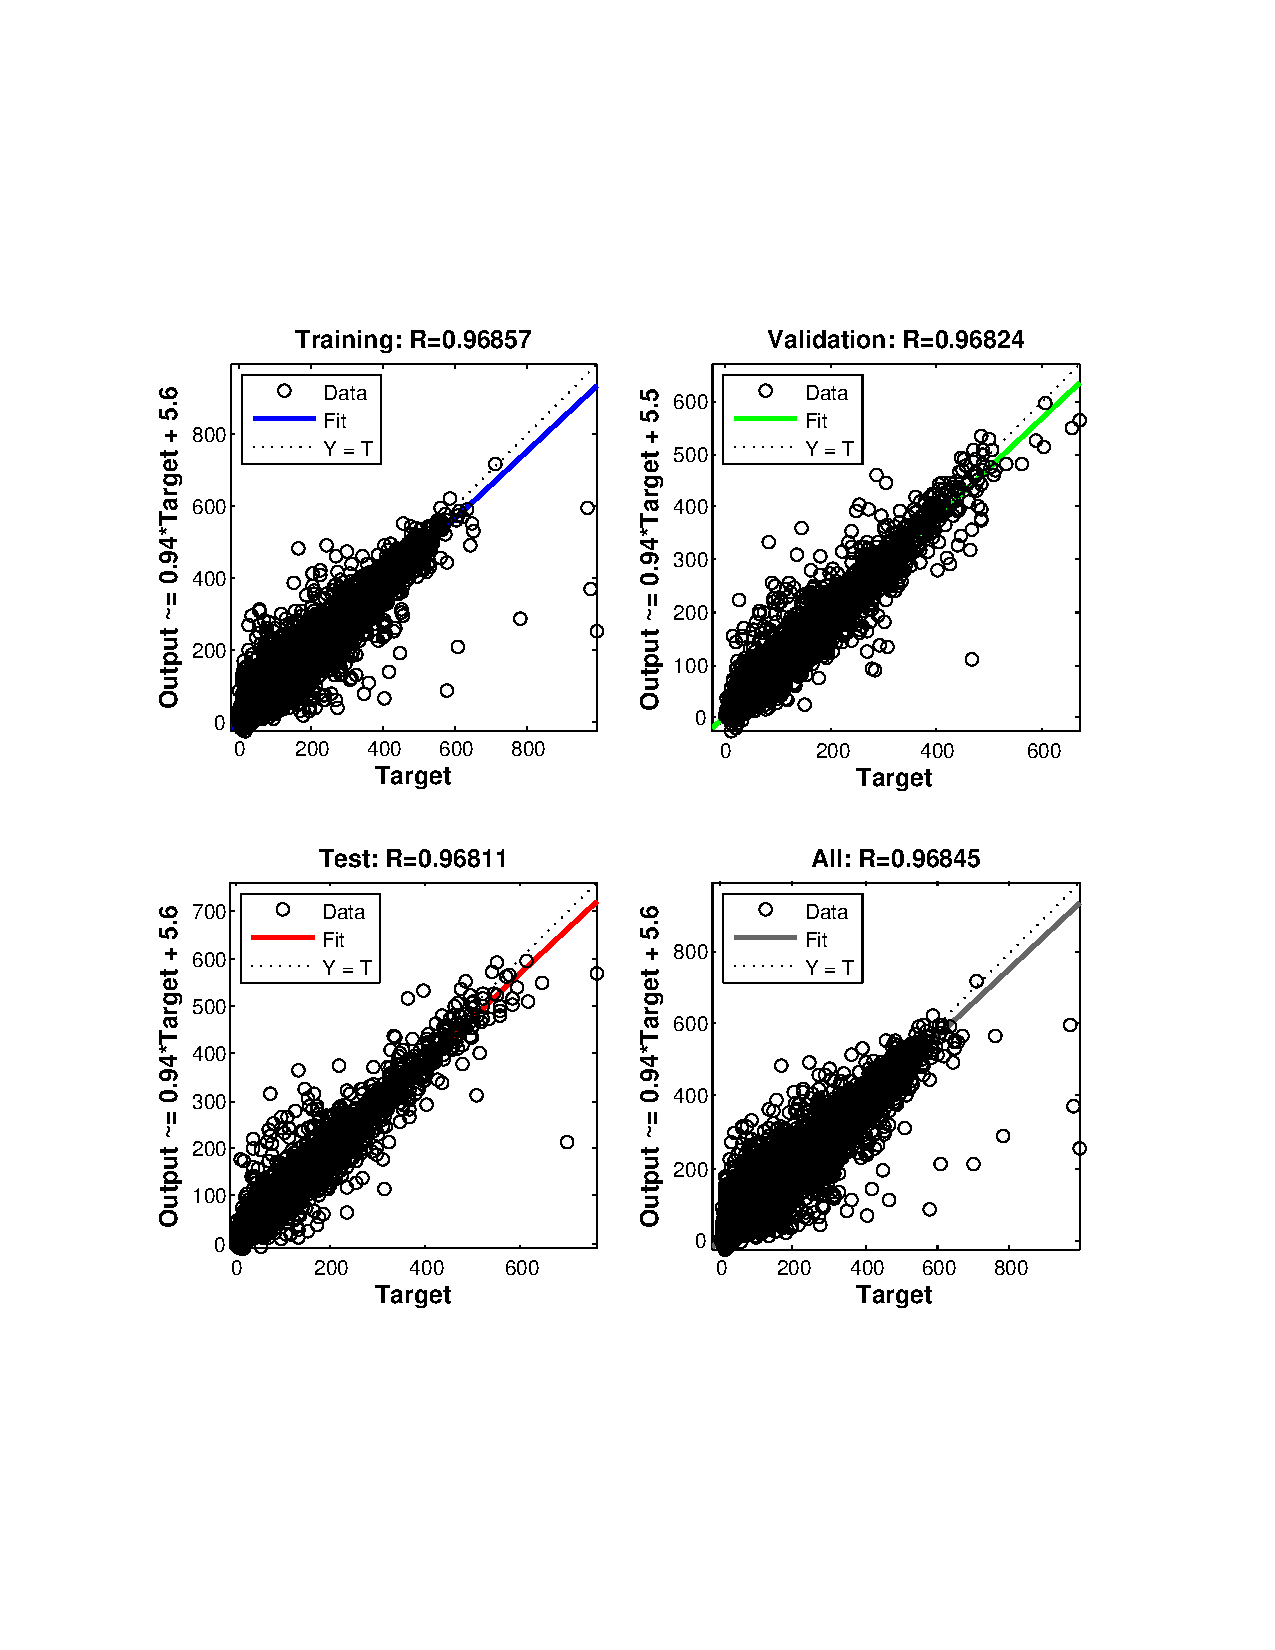
\includegraphics[scale = 0.4, trim = 250 150 250 150]{pic/reg1.pdf}
\caption{The Neural Network fitting using past hours features}
\end{figure}


\begin{figure}[ht]
\centering
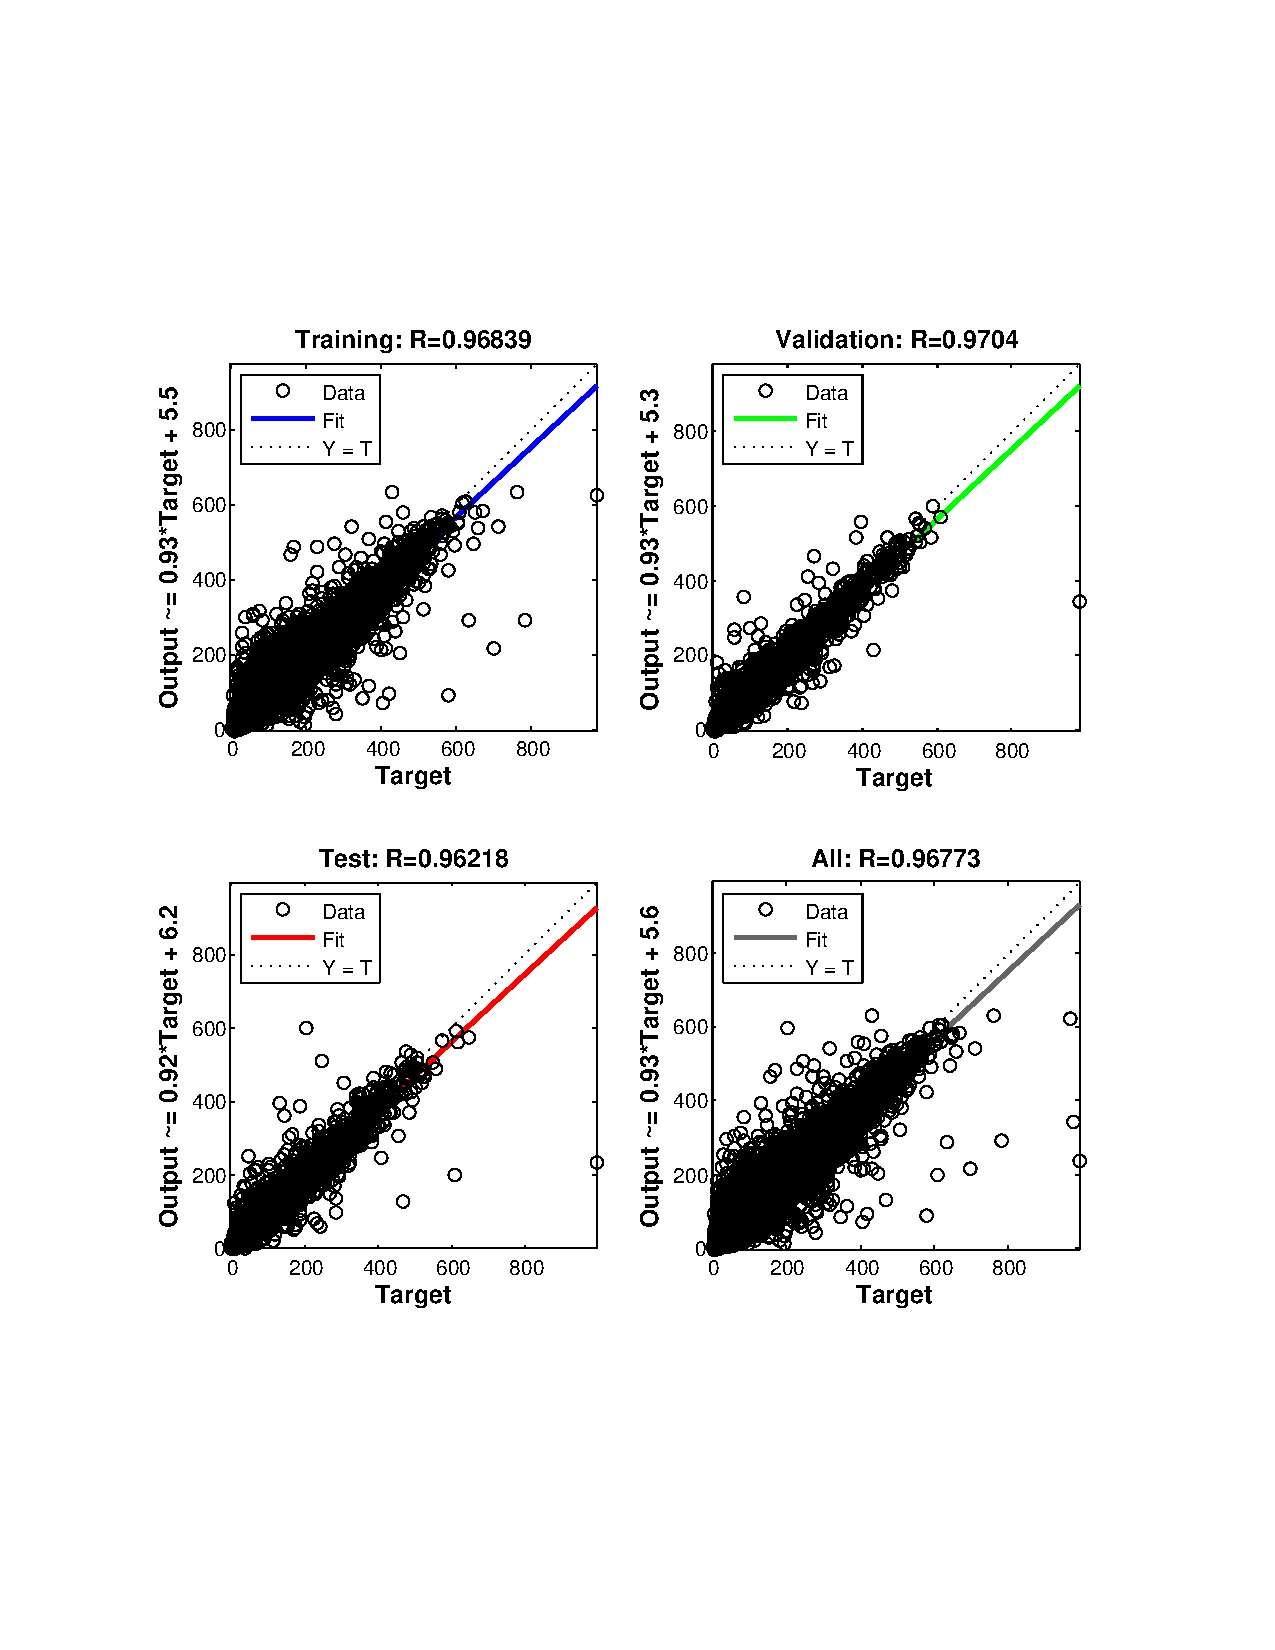
\includegraphics[scale = 0.4, trim = 250 150 250 150]{pic/reg2.pdf}
\caption{The Neural Network fitting using past hours features and same-time past day features}
\end{figure}


As we can see, the two different feature spaces perform well and have a negligible accuracy difference, both with R equals more than 0.95. We can now safe to state that using the local information is quite enough; the PM2.5 value of one time can be sufficiently told from its local information.


In the meantime, I perform a two dimension polynomial regression to see how many hours of past data are sufficient enough. I calculated the Mean Absolute Percentage Error(MAPE) to compare the different dimensions. The result is shown in Figure 3. We can see that using only past two hours features can fit a decent result, further proving the locality property of the PM2.5 value.

\begin{figure}[ht]
\centering
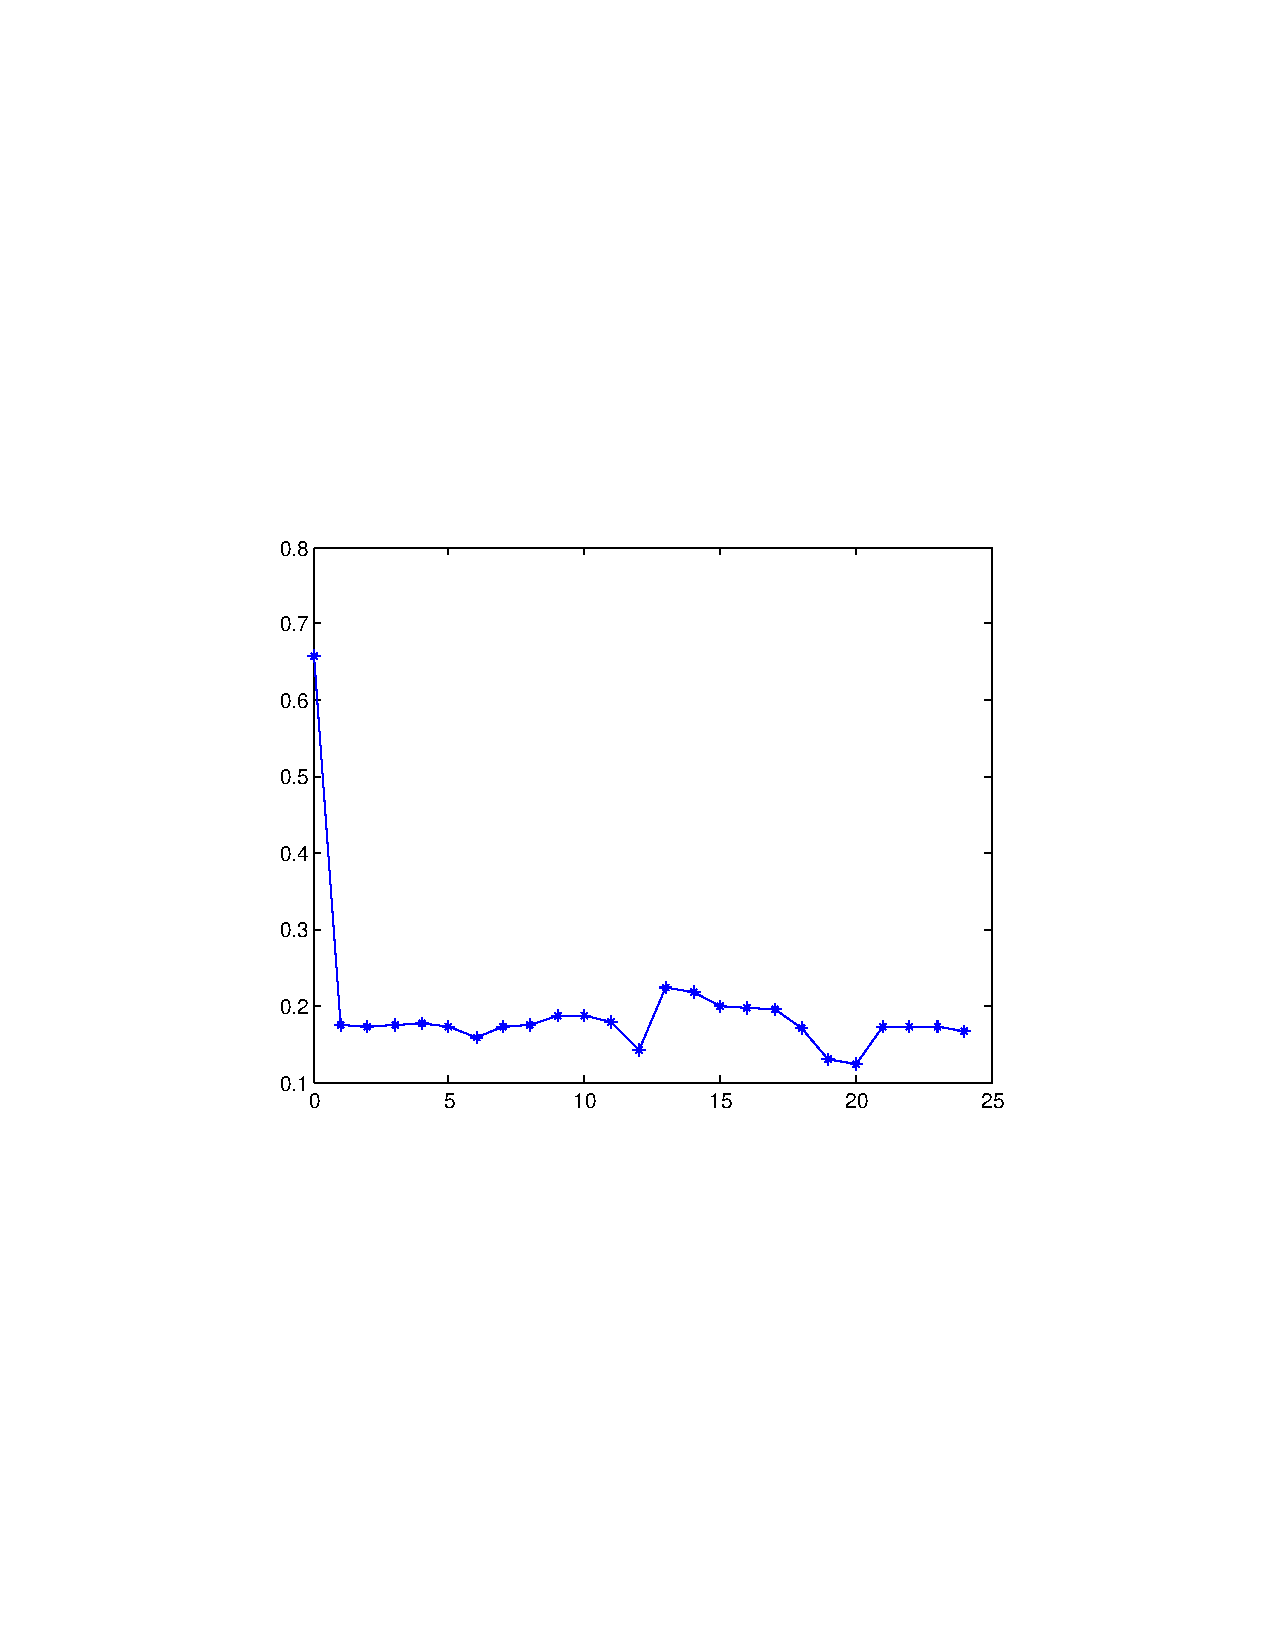
\includegraphics[scale = 0.4, trim = 350 250 350 250]{pic/lg.pdf}
\caption{The MAPE of using data of past x days}
\end{figure}





\subsection{Results for Problem 2}
I now try to solve problem 2 using neural network. I also set 70\% as the training set, 15\% as the cross validation set, and the rest 15\% as the testing set. The neurons in the hidden layer is set to be 20. The experimental results are shown in Figure 4, 5 and 6.
\begin{figure}[ht]
\centering
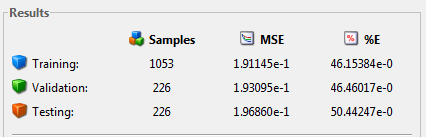
\includegraphics[scale = 0.7]{pic/cl3.png}
\caption{Fitting Results of Problem 2}
\end{figure}

\begin{figure}[ht]
\centering
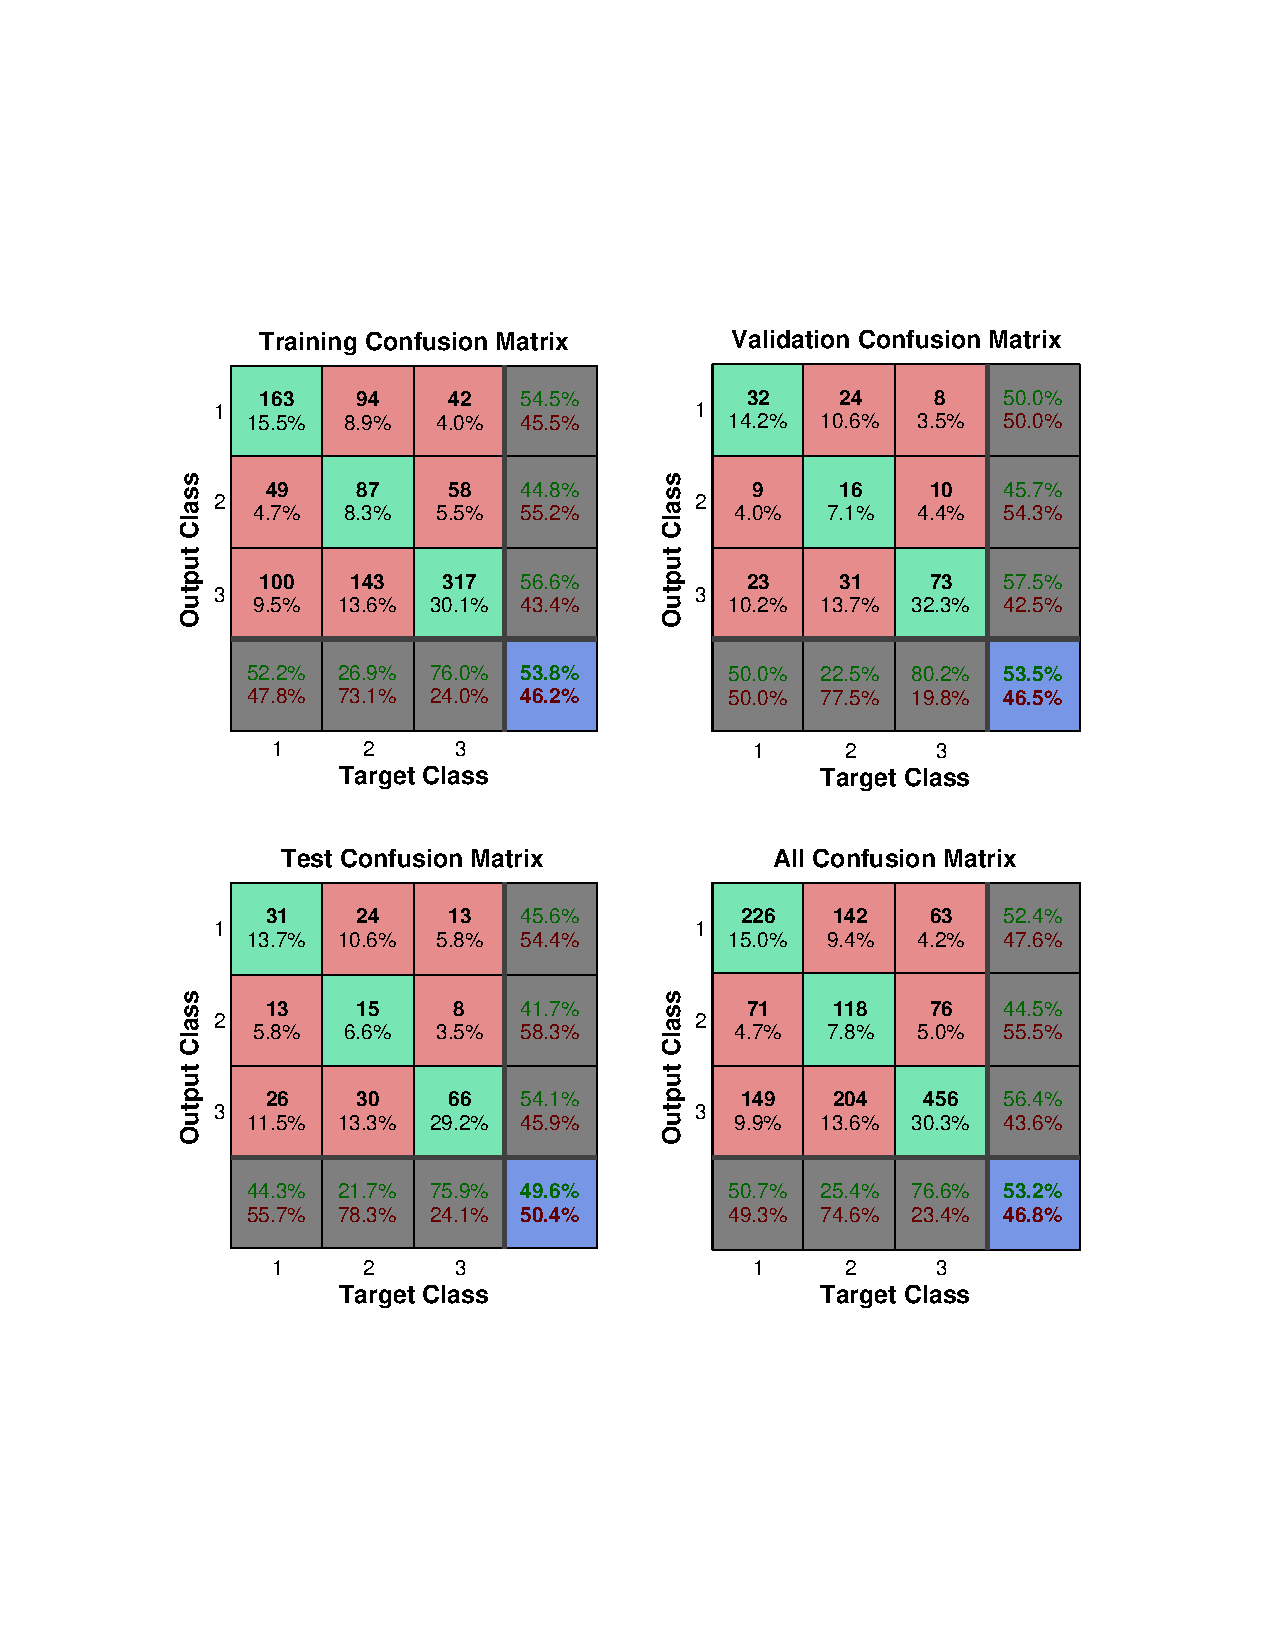
\includegraphics[scale = 0.5, trim = 300 150 300 150]{pic/cl1.pdf}
\caption{The Confusion Matrix}
\end{figure}

\begin{figure}[ht]
\centering
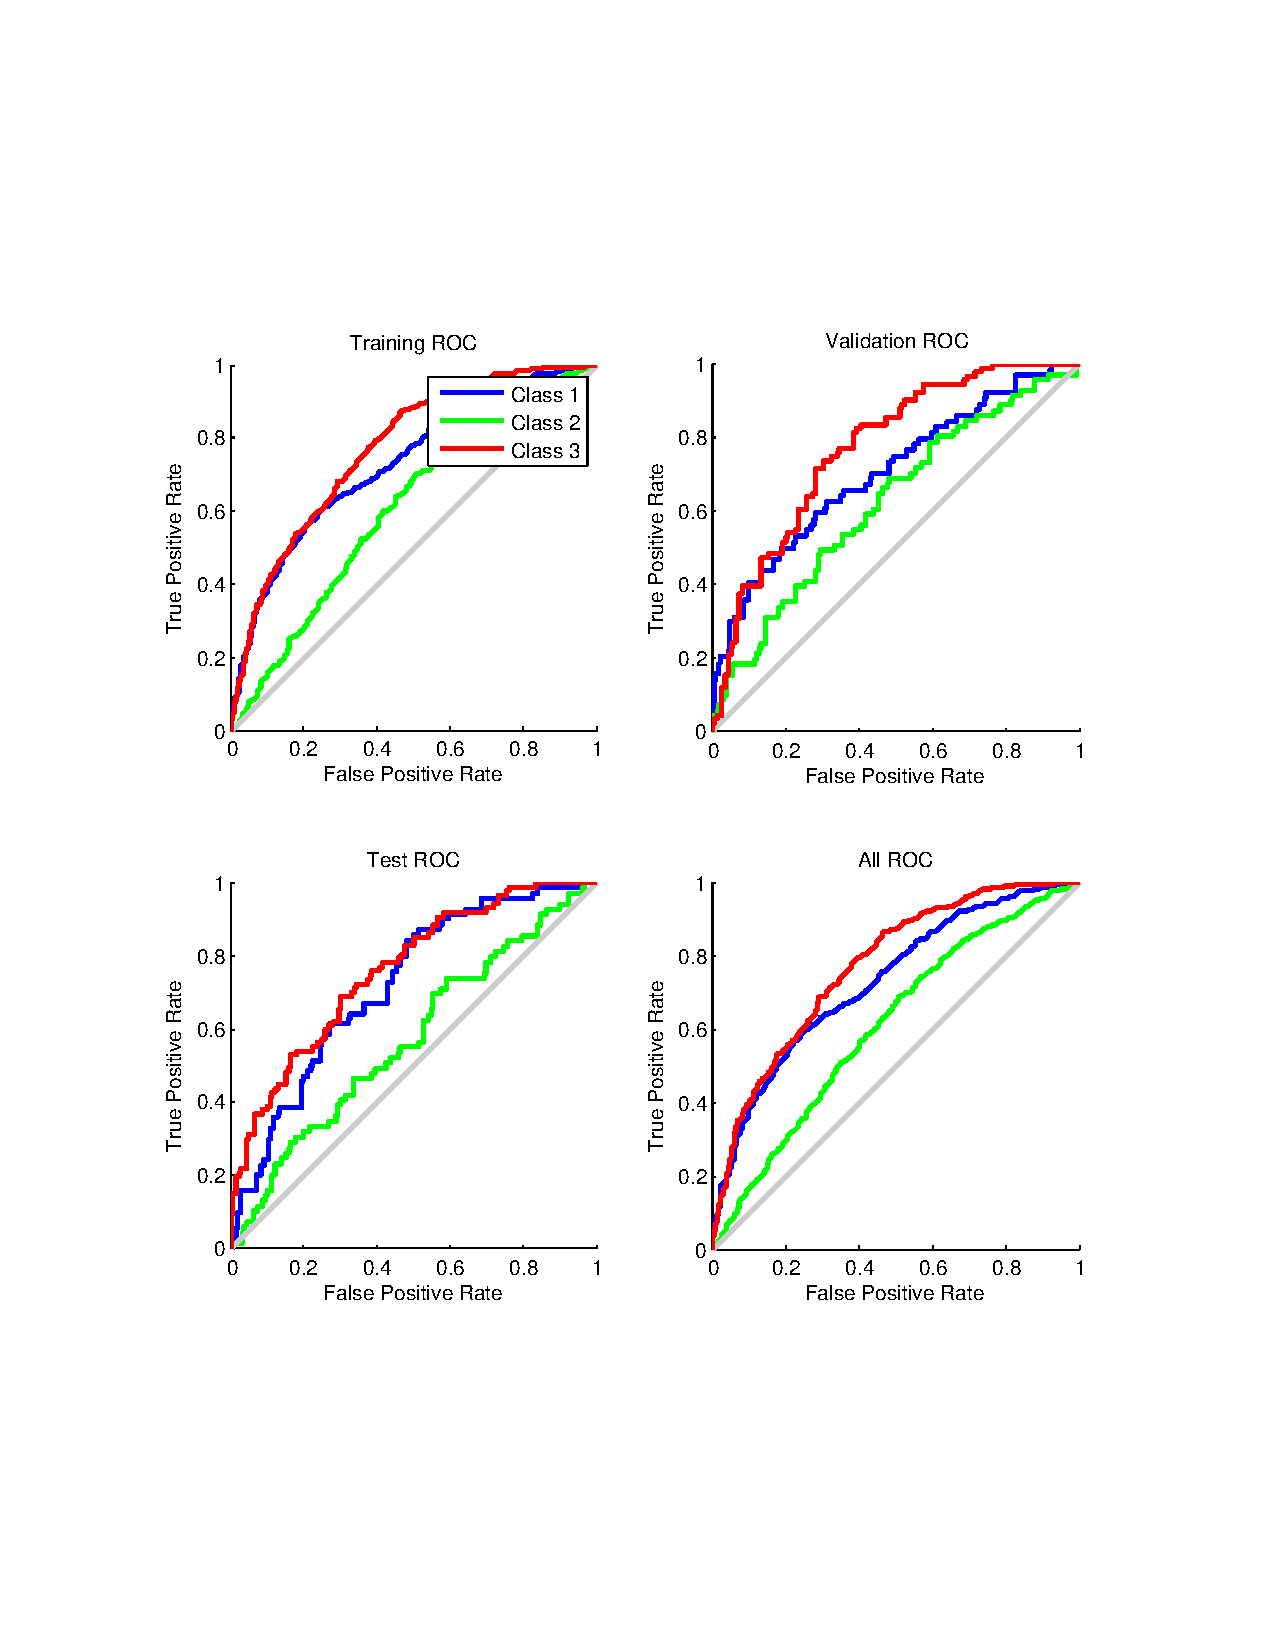
\includegraphics[scale = 0.5, trim = 300 150 300 150]{pic/cl2.pdf}
\caption{The ROC Curve}
\end{figure}

As we can tell, the result is not so good; although the determined data has around 50\% accuracy, which is higher than a random guess, which is 33\%, a lot of input cannot be classified. This is because the amount of training data is so small that I can not introduce a good model. If I have more data, this situation can be solved because we can judge from the result and the shape of the curve that this approach is promising.

\section{Future Work}


Retrospectively, considering all the defects in the whole process, there exist many ways to improve the performance.

\begin{itemize}
    \item The approaches in this paper only considers the past PM value as the features to train the model. Actually, more features can be added to train a better model. For example, I can add the wind strength, precipitation and other meteorological effects. These effects are highly related to the PM2.5 value.
    \item In the previous data selection, I treated every time in a day equally; I trained several uniform models for the whole data. Actually there should have been some difference and the resulting model for each time shall be different. I can thus choose some time in a day to see whether training separately could provide a better result.
    \item I can define other problems and solve them. For example, my friend, Jiaming, aims to predict a long-term value series instead of a single value. This mission, of course, is a far more difficult task, and as far as I know his model does not perform so well according to its complexity. I can try solving that conundrum in future or even propose some more interesting and challenging problems.
\end{itemize}

\section{Conclusions}
The importance of the environment is beyond words. Environment governance is one of the most urgent contemporary issues. Before we can fully emancipate ourselves out of the pollution problems, we can use the cutting-edge data mining techniques to predict the value of some pollution index, and thus take corresponding measures.

In this paper, I lead a roadmap from the beginning to the end. I first give a full description of the PM2.5 problems to be solved in this paper. Next, the Chapter 3 starts from getting the data to processing the data, making a compact, simple feature vector for those built in MATLAB machine learning toolkits.

After these work, some famous models which have been taught in class and have been well built in MATLAB are imposed on the given feature vectors and thus generate different models. I use these disparate models, more concretely, polynomial regression and neural network, to solve the proposed problems, and the corresponding results are given and discussed.

Finally, I make some remarks on the whole approach, indicating some room for further study to improve. Some of them may be easier to realize than others, but each one will benefit the result to some extent after a careful coding and tuning.

%\end{document}  % This is where a 'short' article might terminate
\section{Acknowledgments}
I have learned bunch of knowledge out of this project, including the basics of several machine learning toolkits in MATLAB, the coding tricks, writing the paper\footnote{Actually, I never thought of that writing a paper is such an exhausting and skillful work. From now on I respect more of those 8-page, 10-page paper. It is almost desperate to type so much words.}, so on and so forth. Everything just help me improve and let me become more prepared for my Ph.D career\footnote{YES! I have made up my mind to apply for Ph.D!}. Also, this long journey provides me with a better insight of data mining, which is, and will continue to be, the hottest topic in computer science.

Cannot believe this semester is going to over.  THANK YOU to TAs for a whole semester's great help. THANK YOU to Prof. Yuan for your wonderful instructions. This is a fruitful course and I do deeply feel the elegance of data mining. Hope that everything is alright!

%
% The following two commands are all you need in the
% initial runs of your .tex file to
% produce the bibliography for the citations in your paper.
\bibliographystyle{abbrv}
\bibliography{sigproc}  % sigproc.bib is the name of the Bibliography in this case
% You must have a proper ".bib" file
%  and remember to run:
% latex bibtex latex latex
% to resolve all references
%
% ACM needs 'a single self-contained file'!
%
%APPENDICES are optional
%\balancecolumns

\end{document}
